\documentclass[a4paper,14pt]{article}

% Поддержка русского языка
\usepackage[T1, T2A]{fontenc}    % Кодировка
\usepackage[utf8]{inputenc}  % Кодировка исходного текста
\usepackage[english, russian]{babel}  % Локализация и переносы
\usepackage{titlesec, titletoc} % Для настройки стилей заголовков и содержания
\usepackage{booktabs} % Для использования \toprule, \midrule и \bottomrule
\usepackage{array}  % Для лучшего контроля столбцов
\usepackage{cmap}    % Поиск и копирование в PDF
\usepackage{geometry}    % Поля
    \geometry{left=30mm, right=15mm, top=20mm, bottom=20mm}
\usepackage{hhline} % Для двойных линий и более точного контроля границ
\usepackage{caption} % Для настройки подписей
\usepackage{verbatim}
\usepackage{xcolor} % Пакет для цвета
\usepackage{listings} % Пакет для вставки кода
\usepackage{indentfirst}
\usepackage{graphicx}
\usepackage{float}
\usepackage{amsmath}
\usepackage{tikz}

\usetikzlibrary{shapes.geometric, arrows}

\tikzstyle{startstop} = [rectangle, rounded corners, minimum width=3.5cm, minimum height=1cm, text centered, draw=black, fill=red!30]
\tikzstyle{process} = [rectangle, minimum width=3.5cm, minimum height=1cm, text centered, draw=black, fill=blue!20]
\tikzstyle{decision} = [diamond, minimum width=3.5cm, minimum height=1cm, text centered, draw=black, fill=green!30]
\tikzstyle{arrow} = [thick,->,>=stealth]

% \usepackage{times}

% Установка стандартного отступа (2em)
\setlength{\parindent}{2em}

% Установка отступа после заголовков
\usepackage{titlesec}
\titlespacing*{\section}{0pt}{2\baselineskip}{\baselineskip}
\titlespacing*{\subsection}{0pt}{2\baselineskip}{\baselineskip}
\titlespacing*{\subsubsection}{0pt}{2\baselineskip}{\baselineskip}

% Определение цветов
% \definecolor{operatorcolor}{HTML}{ED028C}
% \definecolor{stringcolor}{HTML}{9400D1}
% \definecolor{commentcolor}{HTML}{005000}
% \definecolor{backgroundcolor}{HTML}{fafafa}
\definecolor{backgroundcolor}{HTML}{fafafa} % Темный фон
\definecolor{keywordcolor}{rgb}{0.86, 0.58, 0.35} % Ключевые слова (оранжевый)
\definecolor{stringcolor}{rgb}{0.72, 0.92, 0.53} % Строки (зеленый)
\definecolor{commentcolor}{HTML}{005000} % Комментарии (серый)
\definecolor{numbercolor}{rgb}{0.75, 0.75, 0.75} % Номера строк (светло-серый)
\definecolor{identifiercolor}{rgb}{0.60, 0.60, 1.00} % Идентификаторы (светло-синий)
\definecolor{keywordtypcolor}{rgb}{0.57, 0.81, 1.00} % Типы данных (голубой)

\captionsetup[table]{justification=raggedright, singlelinecheck=false} % Выравнивание подписи по левому краю

% Установка стиля заголовков разделов: центрирование без номера
\titleformat{\section}[block]{\Large\bfseries\centering}{}{0pt}{}

\title{3.1 Титульный лист}

\begin{document}

\thispagestyle{empty}    % Отключаем колонтитулы

\begin{center}
    ФЕДЕРАЛЬНОЕ ГОСУДАРСТВЕННОЕ АВТОНОМНОЕ ОБРАЗОВАТЕЛЬНОЕ УЧРЕЖДЕНИЕ ВЫСШЕГО ОБРАЗОВАНИЯ\\
    \bfseries{САНКТ-ПЕТЕРБУРГСКИЙ ПОЛИТЕХНИЧЕСКИЙ УНИВЕРСИТЕТ ПЕТРА ВЕЛИКОГО}\\
    Институт компьютерных наук и кибербезопасности\\
    Высшая школа программной инженерии
\end{center}

\vspace{20ex} % Задаем размер вертикального промежутка в явном виде

\begin{center}
    \begin{huge} {\bfseries{\scshape лабораторная работа №1}} \end{huge}

    \vspace{3ex}
    по дисциплине: «Вычислительная матиматика»\\
    Вариант №27
\end{center}

\vspace{30ex}

\noindent Выполнила\\
студентка гр. в5130904/30022\hfill \begin{minipage}{0.6\textwidth} \hfill Г.М.Феллер\end{minipage}

\vspace{3ex}

\noindent Преподаватель \hfill \begin{minipage} {0.6\textwidth}\hfill С.П.Воскобойников\end{minipage}

\vspace{3ex}

\hfill \begin{minipage}{0.6\textwidth} \hfill «\underline{\hspace{1cm}}»\underline{\hspace{3cm}} 2025 г.\end{minipage}

\vfill

\begin{center}
    Санкт-Петербург\\ 
    2025
\end{center}

\newpage % Начинаем новую страницу\

% Отключение нумерации разделов в заголовках разделов и подразделов
\titleformat{\section}[block]{\Large\bfseries\centering}{}{0pt}{}

% Настройка заголовков подразделов с использованием символа "§" и собственной нумерации
\renewcommand{\thesubsection}{\S\arabic{subsection}}
\titleformat{\subsection}[block]{\large\bfseries}{\thesubsection}{1em}{}
% Установка автоматического сброса счетчика подразделов при начале нового раздела

% Определение стиля оглавления
\titlecontents{section}[0pt] % Left indent
{\vspace{0.5ex}\hspace{1em}} % Above code and left spacing
{} % Numbered entry format (empty to remove numbers)
{} % Numberless entry format
{\titlerule*[1pc]{.}\contentspage} % Filler-page format

\newpage


\section{1. Вычислите $||x||_{1}$, $||x||_{2}$, $||x||_{\infty}$ вектора $x = [-3, -5, 2, 4]$}

1. L1-норма
$$
||x||_{1} = \sum_{i=1}^n |x_{i}| = |-3| + |-5| + |2| + |4| = 3 + 5 + 2 + 4 = 14
$$

2. L2-норма
$$
||x||_{2} = \sqrt{ \sum_{i=1}^n x_{i}^2 } = \sqrt{ (-3)^2 + (-5)^2 + 2^2 + 4^2 } = \sqrt{ 9 + 25 + 4 + 16 } = \sqrt{ 54 }
$$

3. L-норма
$$
||x||_{\infty} = \max\limits_{1 \leq i \leq n}|x_{i}| = \max\{|-3|, |-5|, |2|, |4|\} = \max\{3,5,2,4\} = 5
$$

Ответ:
\begin{itemize}
    \item $||x||_{1}=14$
    \item $||x||_{2} = \sqrt{ 54 }$
    \item $||x||_{\infty} = 5$
\end{itemize}

\section{2. Вычислите $||A||_{1}$, $||A||_{\infty}$ матрицы}
$$
A= \begin{bmatrix}
0  & 0  & 0  & 7 \\
7  & 0  & 6  & 5 \\
-8 & -1 & 5  & 6 \\
0  & 2  & -4 & -2
\end{bmatrix}
$$

1. L1-норма
$$
||A||_{1} = \max\limits_{1 \leq j \leq n} \sum_{i=1}^m|a_{ij}|
$$
Столбец 1: $|0| + |7| + |-8| + |0| = 15$\\
Столбец 2: $|0| + |0| + |-1| + |2| = 3$\\
Столбец 3: $|0| + |6| + |5| + |-4| = 15$\\
Столбец 4: $|7|+|5|+|6|+|-2|=20$\\
Максимальная сумма: $\max\{15, 3, 15, 20\} = 20$\\
$||A||_{1} = 20$\\

2. L-норма
$$
||A||_{\infty} = \max\limits_{1 \leq i \leq m} \sum_{j=1}^m|a_{ij}
$$
Строка 1: $|0|+|0|+|0|+|7| = 7$\\
Строка 2: $|7|+|0|+|6|+|5| = 18$\\
Строка 3: $|-8|+|-1|+|5|+|6|=20$\\
Строка 4: $|0|+|2|+|-4|+|-2|=8$\\
Максимальная сумма: $\max\{7, 18, 20, 8\} = 20$\\
$||A||_{\infty}=20$\\

Ответ:
\begin{itemize}
	\item $||A||_{1} = 20$
	\item $||A||_{\infty}=20$
\end{itemize}

\section{3.  Используя $||A||_{1}$ и $||A||_{\infty}$, оцените $|\lambda|_{max}$ для матрицы. Какая норма даёт лучшую оценку?}
$$
A = \begin{pmatrix}
-8 & 3 & 5 & 5 \\
-1 & 4 & 2 & 0 \\
7 & -4 & 3 & 4 \\
7 & 6 & -8 & 7
\end{pmatrix}
$$

Норма $L_{1}$ матрицы $A$ определяется как максимальная сумма абсолютных значений элементов в столбцах:
$$
||A||_{1} = \max\limits_{1 \leq j \leq 4} \sum_{i=1}^4|a_{ij}|
$$
Столбец 1: $|-8|+|-1|+|7|+|7|=23$\\
Столбец 2: $|3|+|4|+|-4|+|6|=17$\\
Столбец 3: $|5|+|2|+|3|+|-8|=18$\\
Столбец 4: $|5|+|0|+|4|+|7|=16$\\
$$||A||_{1}=\max(23, 17, 18, 16)=23$$
Норма $L_{\infty}$ матрицы $A$ определяется как максимальная сумма абсолютных значений элементов в строках:
$$
||A||_{\infty} = \max\limits_{1 \leq i \leq 4} \sum_{j=1}^4|a_{ij}
$$
Строка 1: $|-8|+|3|+|5|+|5|=21$\\
Строка 2: $|-1|+|4|+|2|+|0|=7$\\
Строка 3: $|7|+|-4|+|3|+|4|=18$\\
Строка 4: $|7|+|6|+|-8|+|7|=28$\\
$$||A||_{1}=\max(21, 7, 18, 28)=28$$
Максимальное по модулю собственное значение $\lambda_{max}$ матрицы $A$ можно оценить с помощью норм $L_{1}$ и $L_{\infty}$:
$$
|\lambda_{max}|\leq||A||_{1}=23
$$
$$
|\lambda_{max}|\leq||A||_{\infty}=28
$$
Норма $L_{1}$ дает лучшую оценку максимального по модулю собственного значения:
$$
|\lambda_{max}|\leq23
$$

\section{4. Верно ли утверждение, что матрица, имеющая нулевое собственное значение, вырождена, а значит ее определитель равен нулю?}

Да, утверждение верно. Матрица, имеющая нулевое собствеенное значение, является вырожденной, и ее определитель равен нулю.
Это можно объяснить следующим образом:

1. Собственные значения матрицы связаны с ее определителем. Определитель матрицы равен произведению всех ее собственных значений.

2. Если хотя бы одно собственное значение равно нулю, то произведение всех собственных значений также будет равно нулю.

3. Матрица считается вырожденной, если ее определитель равен нулю.
Таким образом, наличие нулевого собственного значения гарантирует, что матрица вырождена, а ее определитель равен нулю.

\section{5. Какие из трех матриц заведомо невырождены? Указание: Примените теорему Гершгорина для исходной и транспонированной матрицы. Постройте круги Гершгорина для обоих случаев.}
$$
A = \begin{pmatrix}
    4 & 1 & 0 & 2 \\
    -4 & 7 & 0 & 2 \\
    0 & 3 & 6 & 2 \\
    0 & 4 & 0 & 5
    \end{pmatrix}
B = \begin{pmatrix}
    4 & 0 & 1 & 0 \\
    3 & 4 & -3 & 3 \\
    3 & 0 & -3 & 4 \\
    3 & -2 & -2 & 0
    \end{pmatrix}
C = \begin{pmatrix}
    2 & 0 & 1 & 0 \\
    0 & 3 & -4 & -2 \\
    0 & 0 & 6 & 2 \\
    -1 & -2 & 0 & 5
    \end{pmatrix}
$$

Транспонированные матрицы
$$
A^T = \begin{pmatrix}
    4 & -4 & 0 & 0 \\
    1 & 7 & 3 & 4 \\
    0 & 0 & 6 & 0 \\
    2 & 2 & 2 & 5
    \end{pmatrix}
B^T = \begin{pmatrix}
    4 & 3 & 3 & 3 \\
    0 & 4 & 0 & -2 \\
    1 & -3 & -3 & -2 \\
    0 & 3 & 4 & 0
    \end{pmatrix}
C^T = \begin{pmatrix}
    2 & 0 & 0 & -1 \\
    0 & 3 & 0 & -2 \\
    1 & -4 & 6 & 0 \\
    0 & -2 & 2 & 5
    \end{pmatrix}
$$
\paragraph{Проверка строгого диагонального преобладания.\newline}

Строгое диагональное преобладание в матрице означает, что для каждой строки модуль диагонального элемента строго больше суммы модулей всех остальных элементов этой строки:
$$
|a_{ii}| = \sum_{j\ne i}|a_{ij}|
$$

Это условие можно проверить, используя круги Гершгорина:

- Построить круги Гершгорина для матрицы

- Проверить, что для каждого круга его центр (диагональный элемент) находится вне круга. 

Если это условие выполняется для всех кругов, то матрица обладает строгим диагональным преобладанием.\\

Матрица $A$\\
1. Строка 1: $|4| = 4; |1| + |0| + |2| = 3; 4>3$\\
2. Строка 2: $|7| = 7; |-4| + |0| + |2| = 6; 7>6$\\
3. Строка 3: $|6| = 6; |0| + |3| + |2| = 5; 6 > 5$\\
4. Строка 4: $|5| = 5; |0| + |4| + |0| = 4; 5 > 4$\\
Матрица $A$ имеет строгое диагональное преобладание.\\

Транспонированная матрица $A^T$\\
1. Строка 1: $|4| = 4;  |-4| + |0| + |0| = 4; 4 \leq 4$\\
2. Строка 2: $|7| = 7; |1| + |3| + |4| = 8; 7 \leq 8$\\
3. Строка 3: $|6| = 6; |0| + |0| + |0| = 0; 6 > 0$\\
4. Строка 4: $|5| = 5; |2| + |2| + |2| = 6; 5 \leq 6$\\
Транспонированная матрица $A^T$ не имеет строгого диагонального преобладания.\\

Матрица $B$\\
1. Строка 1: $|4|=4; |0| + |1| + |0| = 1; 4 > 1$\\
2. Строка 2: $|4| = 4; |3| + |-3| + |3| = 9; 4 \leq 9$\\
3. Строка 3: $|-3| = 3; |3| + |0| + |4| = 7; 3 \leq 7$\\
4. Строка 4: $|0| = 0; |3| + |-2| + |-2| = 7; 0 \leq 7$\\
Матрица $B$ не имеет строгого диагонального преобладания.\\

Транспонированная матрица $B^T$\\
1. Строка 1: $|4| = 4; |3| + |3| + |3| = 9; 4 \leq 9$\\
2. Строка 2: $|4| = 4; |0| + |0| + |-2| = 2; 4 > 2$\\
3. Строка 3: $|-3| = 3; |1| + |-3| + |-2| = 6; 3 \leq 6$\\
4. Строка 4: $|0| = 0; |0| + |3| + |4| = 7; 0 \leq 7$\\
Транспонированная матрица $B^T$ не имеет строгого диагонального преобладания.\\

Матрица $C$\\
1. Строка 1: $|2| = 2; |0| + |1| + |0| = 1; 2 > 1$\\
2. Строка 2: $|3| = 3; |0| + |-4| + |-2| = 6; 3 \leq 6$\\
3. Строка 3: $|6| = 6; |0| + |0| + |2| = 2; 6 > 2$\\
4. Строка 4: $|5| = 5; |-1| + |-2| + |0| = 3; 5>3$\\
Матрица $C$ не имеет строгого диагонального преобладания.\\

Транспонированная матрица $C^T$\\
1. Строка 1: $|2| = 2; |0| + |0| + |-1| = 1; 2>1$\\
2. Строка 2: $|3| = 3; |0| + |0| + |-2| = 2; 3>2$\\
3. Строка 3: $|6| = 6; |1| + |-4| + |0| = 5; 6 > 5$\\
4. Строка 4: $|5| = 5; |0| + |-2| + |2| = 4; 5>4$\\
Транспонированная матрица $C^T$  имеет строгое диагональное преобладание.\\

Следовательно, матрицы $A$ и $C^T$ имеют строгое диагональное преобладание, значит они заведомо невырождены.

\paragraph{Круги Гершгорина\\\\}

Матрица $A$\\
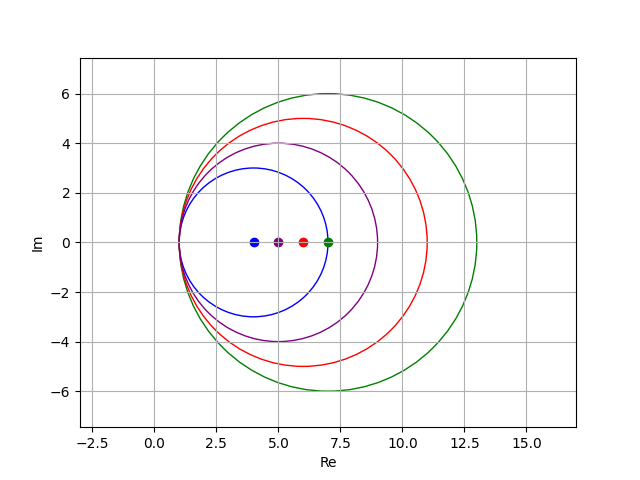
\includegraphics{matrix_a.png}

\newpage
Матрица $A^T$\\
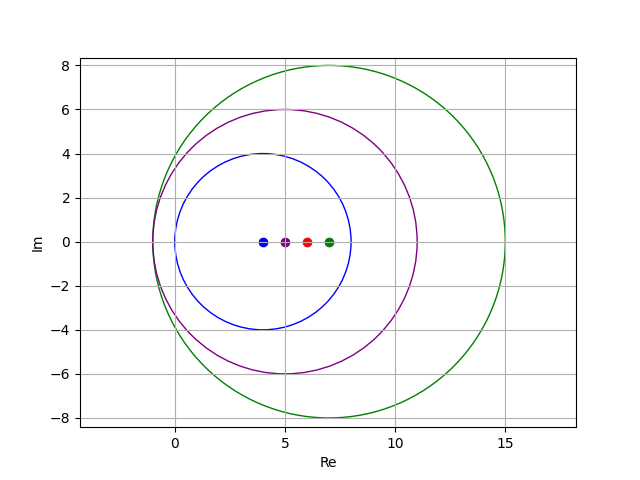
\includegraphics{matrix_at.png}

Матрица $B$\\
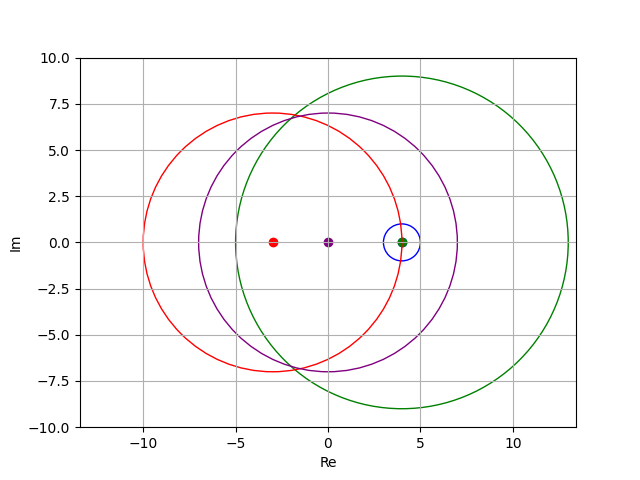
\includegraphics{matrix_b.png}

Матрица $B^T$\\
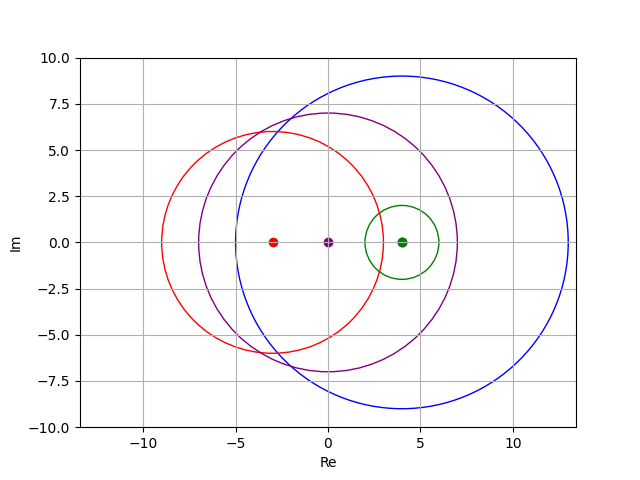
\includegraphics{matrix_bt.png}

Матрица $C$\\
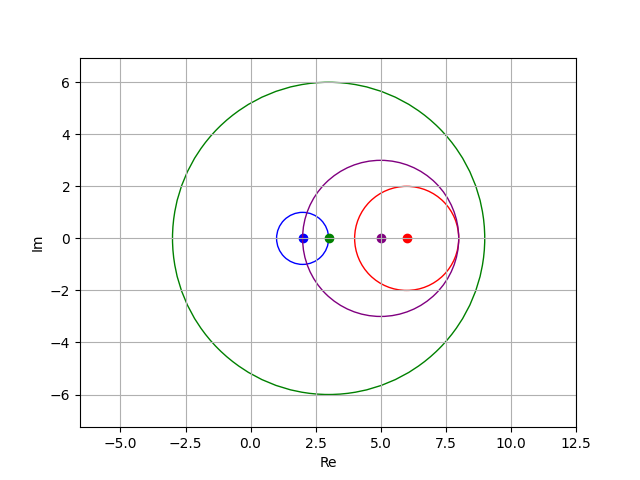
\includegraphics{matrix_c.png}

Матрица $C^T$\\
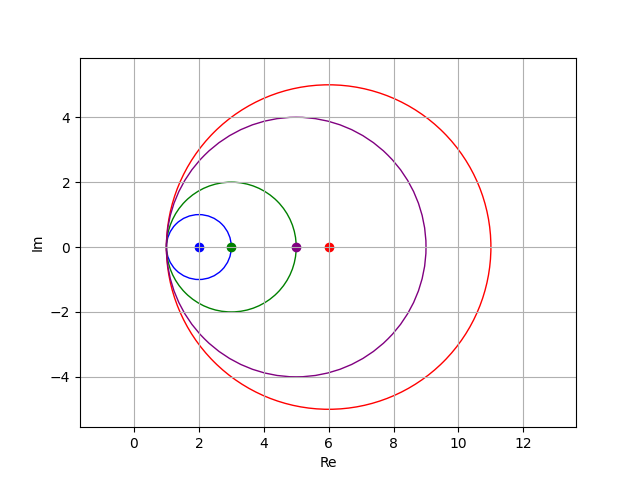
\includegraphics{matrix_ct.png}

\section{6. Для системы уравнений $Ax = b$ вычислите невязку, если известно приближённое решение.}
$$
A = \begin{pmatrix}
    -1 & 1 & -2 & 0 \\
    1 & -2 & -3 & 1 \\
    -1 & -1 & 1 & -4 \\
    3 & 1 & 4 & -2
    \end{pmatrix}
b = \begin{pmatrix}
    -3 \\
    0 \\
    0 \\
    -4
    \end{pmatrix}
x_{approx} = \begin{pmatrix}
    2 \\
    0 \\
    2 \\
    0
    \end{pmatrix}
$$\\
 
Вычисление произведение $Ax_{approx}$
$$
Ax_{approx} = \begin{pmatrix}
    -1 & 1 & -2 & 0 \\
    1 & -2 & -3 & 1 \\
    -1 & -1 & 1 & -4 \\
    3 & 1 & 4 & -2
    \end{pmatrix}
    \begin{pmatrix}
    2 \\
    0 \\
    2 \\
    0
    \end{pmatrix}
    =
    \begin{pmatrix}
    -6 \\
    -4 \\
    0 \\
    14
    \end{pmatrix}
$$\\

Вычисление невязки
$$
r = b - Ax_{approx} = 
    \begin{pmatrix}
    -3 \\
    0 \\
    0 \\
    -4
    \end{pmatrix}
    -
    \begin{pmatrix}
    -6 \\
    -4 \\
    0 \\
    14
    \end{pmatrix}
    =
    \begin{pmatrix}
    3 \\
    4 \\
    0 \\
    18
    \end{pmatrix}
$$

\section{7. Для матрицы $A$ напишите матрицу перестановки $P$ второй и четвертой строк. Чем будет отличаться матрица $PA$ от $AP$?}
$$
A = \begin{pmatrix}
2 & 0 & 2 & 0 \\
3 & 2 & 0 & 0 \\
1 & -3 & 4 & 0 \\
1 & 4 & 2 & -4
\end{pmatrix}
$$\\

Матрица перестановок $P$, которая переставляет вторую и четвертую строки имеет вид:
$$
P_{24} = \begin{pmatrix}
1 & 0 & 0 & 0 \\
0 & 0 & 0 & 1 \\
0 & 0 & 1 & 0 \\
0 & 1 & 0 & 0
\end{pmatrix}
$$

Умножение $P_{24}A$ переставляет строки матрицы $A$:
$$
P_{24}A = \begin{pmatrix}
        1 & 0 & 0 & 0 \\
        0 & 0 & 0 & 1 \\
        0 & 0 & 1 & 0 \\
        0 & 1 & 0 & 0
    \end{pmatrix}
    \begin{pmatrix}
        2 & 0 & 2 & 0 \\
        3 & 2 & 0 & 0 \\
        1 & -3 & 4 & 0 \\
        1 & 4 & 2 & -4
    \end{pmatrix}
    = 
    \begin{pmatrix}
        2 & 0 & 2 & 0 \\
        1 & 4 & 2 & -4 \\
        1 & -3 & 4 & 0 \\
        3 & 2 & 0 & 0
    \end{pmatrix}
    $$

Умножение $AP_{24}$ переставляет столбцы матрицы $A$:
$$
AP_{24} = \begin{pmatrix}
        2 & 0 & 2 & 0 \\
        3 & 2 & 0 & 0 \\
        1 & -3 & 4 & 0 \\
        1 & 4 & 2 & -4
    \end{pmatrix}
    \begin{pmatrix}
        1 & 0 & 0 & 0 \\
        0 & 0 & 0 & 1 \\
        0 & 0 & 1 & 0 \\
        0 & 1 & 0 & 0
    \end{pmatrix}
    = 
    \begin{pmatrix}
        2 & 0 & 2 & 0 \\
        3 & 0 & 0 & 2 \\
        1 & 0 & 4 & -3 \\
        1 & -4 & 2 & 4
    \end{pmatrix}
    $$

\section{8. Для матрицы $A$ напишите матрицу исключения $E$, обнуляющую в первом столбце все элементы, начиная со второго. Вычислите произведение $ЭА$. Вычисления провести в простых дробях.}
$$
A = \begin{pmatrix}
5 & 0 & 2 & 3 \\
0 & 6 & -4 & -4 \\
-4 & -3 & 11 & 0 \\
0 & 2 & -4 & 8
\end{pmatrix}
$$

Матрица исключения $E$:
$$
E = \begin{pmatrix}
    1 & 0 & 0 & 0 \\
    0 & 1 & 0 & 0 \\
    4/5 & 0 & 1 & 0 \\
    0 & 0 & 0 & 1
\end{pmatrix}
$$

Произведение $EA$:
$$
EA = \begin{pmatrix}
    1 & 0 & 0 & 0 \\
    0 & 1 & 0 & 0 \\
    4/5 & 0 & 1 & 0 \\
    0 & 0 & 0 & 1
\end{pmatrix}
\begin{pmatrix}
    5 & 0 & 2 & 3 \\
    0 & 6 & -4 & -4 \\
    -4 & -3 & 11 & 0 \\
    0 & 2 & -4 & 8
\end{pmatrix}
=
\begin{pmatrix}
    5 & 0 & 2 & 3 \\
    0 & 6 & -4 & -4 \\
    0 & -3 & 63/5 & 12/5 \\
    0 & 2 & -4 & 8
\end{pmatrix}
$$

\section{9. Для матрицы $A$ напишите матрицу Хаусхолдера $Н$, обнуляющую в первом столбце все элементы, начиная со второго. Вычислите произведение $HA$. Вычисления провести в простых дробях с использованием радикалов. При вычислении матриц $H$ используйте знак $+$. Окончательный вид матрицы $H$ вычислите с 7-ю десятичными знаками.}
$$
A = \begin{pmatrix}
5 & 0 & 2 & 3 \\
0 & 6 & -4 & -4 \\
-4 & -3 & 11 & 0 \\
0 & 2 & -4 & 8
\end{pmatrix}
$$

Вектор $u$, который зануляет все элементы столбца, начиная со второго:
$$
u_1 = a + ||a||e_1
$$

Первый столбец матрицы $A$:
$$
a = \begin{pmatrix}
5 \\
0 \\
-4 \\
0 
\end{pmatrix}
$$

$||a||_2 = \sqrt{5^2 + 0^2 + (-4)^2 + 0^2} = \sqrt{25+16} = \sqrt{41}$

$$
e_1 = \begin{pmatrix}
    1 \\
    0 \\
    0 \\
    0
\end{pmatrix}
$$

$$
u_1 = \begin{pmatrix}
        5 \\
        0 \\
        -4 \\
        0 
    \end{pmatrix}
    + 
    \sqrt{41}\begin{pmatrix}
        1 \\
        0 \\
        0 \\
        0
    \end{pmatrix}
    =
    \begin{pmatrix}
        5 + \sqrt{41} \\
        0 \\
        -4 \\
        0
    \end{pmatrix}
$$

Вычислим матрицу Хаусхолдера $H$:
$$
H = I - 2{{u_1u^T}\over{u^Tu_1}}
$$

$$
u^Tu_1 = (5 + \sqrt{41}^2) + 0^2 + (-4)^2 + 0^2 = 82 + 10\sqrt{41}
$$

$$
u_1u^T = \begin{pmatrix}
            5 + \sqrt{41} \\
            0 \\
            -4 \\
            0
        \end{pmatrix}
        \times
        \begin{pmatrix}
            5 + \sqrt{41} & 0 & -4 & 0
        \end{pmatrix}
        =
        \begin{pmatrix}
            66 + 10\sqrt{41} & 0 & -20 - 4\sqrt{41} & 0 \\
            0                & 0 & 0                & 0 \\
            -20 - 4\sqrt{41} & 0 & 16               & 0 \\
            0                & 0 & 0                & 0
        \end{pmatrix}
$$

$$
H = I - 2{{\begin{pmatrix}
            66 + 10\sqrt{41} & 0 & -20 - 4\sqrt{41} & 0 \\
            0                & 0 & 0                & 0 \\
            -20 - 4\sqrt{41} & 0 & 16               & 0 \\
            0                & 0 & 0                & 0
        \end{pmatrix}}\over{82+10\sqrt{41}}}
$$

Упростим:
$$
H =     \begin{pmatrix}
            1 & 0 & 0 & 0 \\
            0 & 1 & 0 & 0 \\
            0 & 0 & 1 & 0 \\
            0 & 0 & 0 & 1
        \end{pmatrix}
        - 2 {\begin{pmatrix}
                66 + 10\sqrt{41} & 0 & -20 - 4\sqrt{41} & 0 \\
                0                & 0 & 0                & 0 \\
                -20 - 4\sqrt{41} & 0 & 16               & 0 \\
                0                & 0 & 0                & 0
            \end{pmatrix}\over{82+10\sqrt{41}}}
$$

После вычислений получаем:
$$
H =     \begin{pmatrix}
            -{5}\over{\sqrt{41}} & 0 & {4}\over{\sqrt{41}} & 0 \\
            0 & 1 & 0 & 0 \\
            {4}\over{\sqrt{41}} & 0 & {5}\over{\sqrt{41}} & 0 \\
            0 & 0 & 0 & 1
        \end{pmatrix}
$$

Произведение $HA$:
$$
HA = \begin{pmatrix}
        -{5}\over{\sqrt{41}} & 0 & {4}\over{\sqrt{41}} & 0 \\
        0 & 1 & 0 & 0 \\
        {4}\over{\sqrt{41}} & 0 & {5}\over{\sqrt{41}} & 0 \\
        0 & 0 & 0 & 1
    \end{pmatrix}
    \begin{pmatrix}
        5 & 0 & 2 & 3 \\
        0 & 6 & -4 & -4 \\
        -4 & -3 & 11 & 0 \\
        0 & 2 & -4 & 8
    \end{pmatrix} = 
    \begin{pmatrix}
        -\sqrt{41} & {12}\over{\sqrt{41}} & -{10}\over{\sqrt{41}} & -{15}\over{\sqrt{41}} \\
        0 & 6 & -4 & -4 \\
        0 & -{18}\over{\sqrt{41}} & {50}\over{\sqrt{41}} & {12}\over{\sqrt{41}} \\
        0 & 2 & -4 & 8
    \end{pmatrix}
$$

Окончательный вид матрицы $H$ c 7-ю десятичными знаками:
$$
H = \begin{pmatrix}
        -0,7808688 & 0 & 0,6246950 & 0 \\
        0          & 1 & 0         & 0 \\
        0,6246950  & 0 & 0,7808688 & 0 \\
        0          & 0 & 0         & 1
    \end{pmatrix}
$$

\section{10. Для матрицы $A$ напишите цепочку матриц Гивенса, обнуляющую в первом столбце все элементы, начиная со второго. В формулах для матриц Гивенса используйте знак + для $c$ и - для $s$. Вычислите произведение последовательности матриц Гивенса и произведение этой матрицы на матрицу $A$. Вычисления провести в простых дробях с использованием радикалов. Окончательный вид матрицы $G$ вычислите с 7-ю десятичными знаками.}
$$
A = \begin{pmatrix}
5 & 0 & 2 & 3 \\
0 & 6 & -4 & -4 \\
-4 & -3 & 11 & 0 \\
0 & 2 & -4 & 8
\end{pmatrix}
$$

Для обнуления элементов первого столбца матрицы \( A \), начиная со второго, с использованием матриц Гивенса, выполним следующие шаги:

1. Обнулим элемент \( a_{31} = -4 \):

   Матрица Гивенса \( G_1 \) для обнуления элемента \( a_{31} \):
   \[
   G_1 = \begin{pmatrix}
   c_1 & 0 & -s_1 & 0 \\
   0 & 1 & 0 & 0 \\
   s_1 & 0 & c_1 & 0 \\
   0 & 0 & 0 & 1
   \end{pmatrix}
   \]
   Где:
   \[
   c_1 = \frac{5}{\sqrt{5^2 + (-4)^2}} = \frac{5}{\sqrt{25 + 16}} = \frac{5}{\sqrt{41}}
   \]
   \[
   s_1 = \frac{4}{\sqrt{41}}
   \]

   Применим \( G_1 \) к \( A \):
   \[
   G_1 A = \begin{pmatrix}
   \frac{5}{\sqrt{41}} & 0 & -\frac{4}{\sqrt{41}} & 0 \\
   0 & 1 & 0 & 0 \\
   \frac{4}{\sqrt{41}} & 0 & \frac{5}{\sqrt{41}} & 0 \\
   0 & 0 & 0 & 1
   \end{pmatrix}
   \begin{pmatrix}
   5 & 0 & 2 & 3 \\
   0 & 6 & -4 & -4 \\
   -4 & -3 & 11 & 0 \\
   0 & 2 & -4 & 8
   \end{pmatrix}
   \]
   \[
   G_1 A = \begin{pmatrix}
   \sqrt{41} & \frac{12}{\sqrt{41}} & -\frac{10}{\sqrt{41}} & \frac{15}{\sqrt{41}} \\
   0 & 6 & -4 & -4 \\
   0 & -\frac{18}{\sqrt{41}} & \frac{50}{\sqrt{41}} & \frac{12}{\sqrt{41}} \\
   0 & 2 & -4 & 8
   \end{pmatrix}
   \]



\section{11. Являются ли матрицы. обнуляющие элементы первого столбца из задачи 9 и задачи 10, одинаковыми?}

Матрицы, обнуляющие элементы первого столбца из задачи 9 и задачи 10 не являются одинаковыми.

\end{document}